
\فصل{پروتکل پیشنهادی}

در این فصل به ارائه‌ی پروتکل پیشنهادی خود برای مسیریابی در شبکه‌های مبتنی بر داده‌های نام‌گذاری شده می‌پردازیم. لازم به ذکر است همان‌طور که پیش‌تر در توضیح دامنه‌ی ارسال مسیریاب‌های NDN به آن اشاره شد، به دلیل انعطاف‌پذیر بودن و پشتیبانی از چندمسیری در این دامنه‌، بسیاری از مشکلات پیش آمده در تحویل بسته‌ها در همین دامنه مدیریت می‌شود و در نتیجه بخشی از انتظارات از قسمت مسیریابی برداشته می‌شود. به عنوان مثال اطمینان از ایجاد نشدن حلقه در مسیرها از مهم‌ترین ویژگی‌های یک پروتکل مسیریابی در شبکه‌های مبتنی بر IP می‌باشد،در حالی که به دلیل معماری NDN در دامنه‌ی ارسال از ایجاد حلقه جلوگیری می‌شود و این مسئله دیگر در نیازمندی‌های دامنه‌ی مسیریابی نیست. 

 با توجه به ساختار شبکه‌های NDN، هر پروتکلی که بخواهد روی این شبکه اجرا شود باید به چهار سوال مهم در مورد موضوعات زیر پاسخ دهد:
\شروع{فقرات}
\فقره \مهم{نام‌گذاری}: چگونگی نام‌گذاری مسیریاب‌ها، پیوند‌ها، و پیغام‌های مسیریابی
\فقره \مهم{مدل اعتماد\زیرنوشت{Trust Model}}: چگونگی توزیع کلید‌های رمز مسیریاب‌ها و اطمینان از صحت آن‌ها
\فقره \مهم{انتشار اطلاعات}: چگونگی انتشار پیغام‌های به‌روزرسانی مسیریابی در سرتاسر شبکه
\فقره \مهم{چندمسیری}: چگونگی پیدا کردن مسیرهای مختلف به یک پیشوند و رتبه‌بندی آن‌ها برای پشتبانی از چندمسیری
\پایان{فقرات}

در ادامه، از میان چهار موضوع بالا، در مورد نام‌گذاری، نحوه‌ی انتشار اطلاعات، و پشتیبانی از چندمسیری در پروتکل پیشنهادی خود صحبت خواهیم کرد. طراحی مدل اعتماد به دلیل داشتن  پیش‌نیازهایی فراوان به آینده موکول خوهد شد. هم‌چنین در مورد پروتکل Sync و نحوه‌ی استفاده از آن برای توزیع بسته‌ها، کشف شکست و ترمیم، و نیز مسئله‌ی شمارش بی‌انتها\زیرنوشت{Count to Infinity Problem} توضیح خواهیم داد.

\قسمت{نام‌گذاری}

یکی از بخش‌های مهم در پروتکل مسیریابی، تعیین نام‌گذاری مسیریاب‌ها و پیغام‌هاست. از آن جایی که مبنای شبکه‌های NDN داده‌های نام‌گذاری شده است، اگر یک پروتکل مسیریابی بخواهد به طور مستقیم روی این شبکه‌ها اجرا شود نیازمند مکانیزم نام‌گذاری متناسب با آن‌هاست. در این بخش به توضیح نام‌گذاری مسیریاب‌ها و پیشوند پیغام‌ها می‌پردازیم و نحوه‌ی نام‌گذاری دقیق‌تر پیغام‌ها را در بخش بعدی بررسی خواهیم کرد. 

با توجه به ساختار سلسله‌مراتبی شبکه، به نظر می‌رسد نام‌گذاری سلسله‌مراتبی مناسب‌ترین گزینه برای بیان ارتباط بین مولفه‌های مختلف آن باشد. بدین منظور برای هر شبکه و هر مسیریاب یک نام در نظر می‌گیریم و کافی است که نام شبکه‌ها و نیز نام مسیریاب‌ها در هر شبکه یکتا باشند. در آن صورت می‌توانیم یک مسیریاب را با نام سلسله‌مراتبی \کج{ /<network>/<router>} بشناسیم که در آن \کج{<network>} نام شبکه و \کج{<router>} نام مسیریاب است. به عنوان مثال نام یک مسیریاب در دانشگاه شریف می‌تواند \کج{/sharif/ce-router} باشد. 

در مورد نام‌گذاری پیغام‌ها باید به این نکته توجه کرد که استفاده از مخزن CCNx مستلزم این است که نام داده‌های یک مجموعه در پیشوندی که نام مجموعه است مشترک باشند. به همین دلیل برای تمام بسته‌های مربوط به مسیریابی از پیشوند \کج{/<network>/RM} استفاده می‌کنیم که در آن \کج{<network>} نام شبکه است و \کج{RM} مخفف Routing Message و برای متمایز کردن بسته‌های مسیریابی از سایر بسته‌هاست. در ادامه‌ی نام هر بسته نوع آن، نام مسیریاب تولید کننده‌ی آن، و عدد نسخه‌ی آن قرار می‌گیرند. در بخش‌های بعدی در مورد نوع بسته‌ها و نسخه‌بندی آن‌ها بیشتر توضیح خواهیم داد.

\قسمت{پیغام‌ها}

به دلیل مستقل شدن داده از مکان آن در شبکه‌های NDN، به دو نوع مسیریابی در این شبکه‌ها نیازمندیم، یک نوع مسیریابی برای یافتن تولید‌کننده‌های یک پیشوند خاص، و نوع دیگری از مسیریابی برای پیدا کردن مسیرهای بین مسیریاب‌ها برای پاسخ دادن به بسته‌های درخواست. همان‌طور که در فصل  ~\ref{prevWorks} دیدیم، بعضی از پروتکل‌های پیشنهادی برای جداکردن این دو مسیریابی از معماری دو لایه استفاده کرده‌اند تا یک لایه به نگهداری و به‌روزرسانی توپولوژی شبکه بپردازد و دیگری به توزیع پیشوند‌ها. در سایر پروتکل‌ها این جداسازی، با تفکیک بسته‌های مسیریابی پرداخته‌اند تا هر نوع بسته اطلاعات مربوط به نوع مسیریابی خاصی را در شبکه توزیع کند. ما نیز راه حل دوم را پیش می‌گیریم و دو نوع بسته‌ی مسیریابی تعریف می‌کنیم. بسته‌های نوع اول در فرآیندی مشابه پروتکل‌های مبتنی بر فاصله، اطلاعات مربوط به مسیرهای بین مسیریاب‌ها را حمل می‌کنند که آن‌ها را اعلام‌کننده‌ی فاصله\زیرنوشت{Distance Announcement} (DA) می‌نامیم. بسته‌های نوع دوم حاوی اطلاعات مربوط به پیشوند‌ها و تولید‌کنندگان آن‌ها هستند که اعلام‌کننده‌ی پیشوند\زیرنوشت{Prefix Announcement} (PA) نامیده شده‌اند. 
\begin{figure}[hb!]
\centering
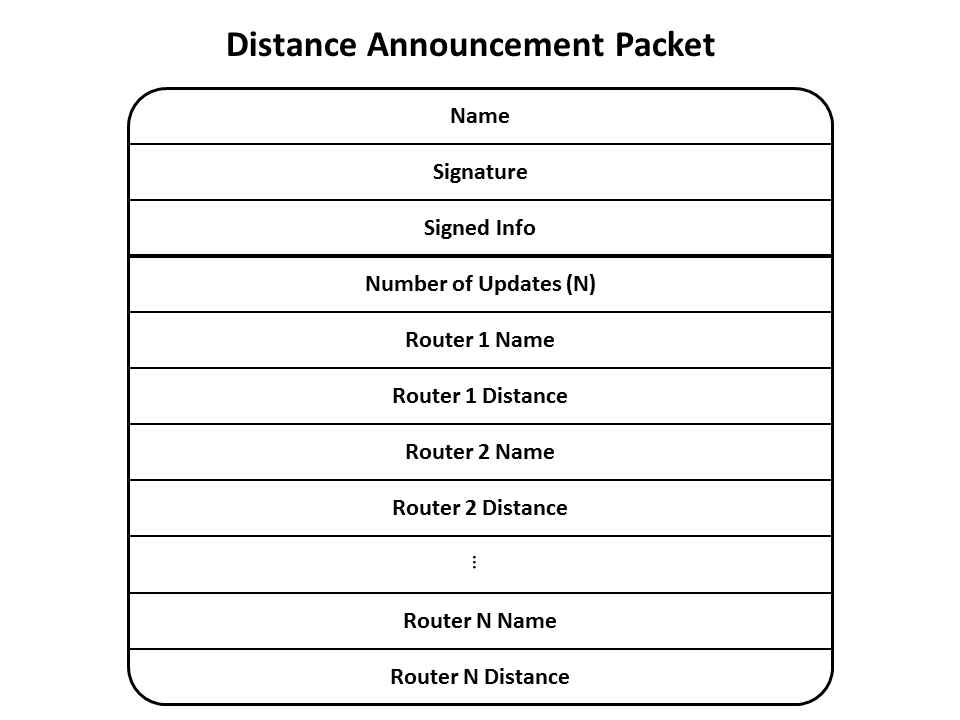
\includegraphics[scale=0.6]{./resources/figures/DA.png}
\caption{محتویات بسته‌ی اعلام‌کننده‌ی فاصله}
\label{fig:DA}
\end{figure}

بسته‌های DA با نام \کج{/<network>/RM/<router>/DM} مشخص می‌شوند که در آن \کج{<router>} نام مسیریابی است که این بسته را تولید کرده است و \کج{<network>} نام شبکه‌ی آن است. محتویات این بسته را در شکل ~\ref{fig:DA} مشاهده می‌کنید. پس از سرآیند بسته‌ی داده‌ی NDN، ابتدا تعداد به روزرسانی‌ها مشخص می‌شود. سپس به ازای هر به روزرسانی نام مسیریابی که فاصله‌ی آن تغییر کرده است به همراه فاصله‌ی جدید آن قرار می‌گیرد. لازم به ذکر است که در ابتدای راه‌اندازی مسیریاب، این فاصله‌ها تنها برای همسایه‌های آن تعریف شده‌اند، و پس از دریافت پیغام‌های به روزرسانی از بقیه‌ی مسیریاب‌های شبکه، فاصله تا دیگر مسیریاب‌ها نیز مشخص می‌شوند. هم‌چنین هر مسیریاب تنها بهترین مسیرهای خود تا دیگر مسیریاب‌ها را به دیگران اعلام می‌کند. همان‌طور که در قسمت ‍~\ref{multipach} خواهیم گفت، هر مسیریاب با دریافت DA از همسایگان خود، مسیرهای متفاوت را برای مقصد‌های یکسان در نظر می‌گیرد و در FIB ذخیره می‌کند.


\begin{figure}[hb!]
\centering
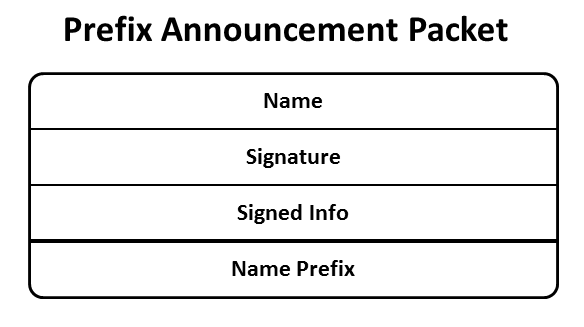
\includegraphics[scale=0.6]{./resources/figures/PA.png}
\caption{محتویات بسته‌ی اعلام‌کننده‌ی پیشوند}
\label{fig:PA}
\end{figure}

بسته‌های نوع دوم که PA نام دارند با \کج{<network>/RM/PA/<router>/ID.<ID>} مشخص می‌شوند که مشابه بسته‌های PA در آن \کج{<router>} و \کج{<network>} به ترتیب نام مسیریاب تولیدکننده‌ی بسته و شبکه‌ی آن هستند. محتویات این بسته را می‌توانید در شکل ~\ref{fig:PA} مشاهده کنید. در بخش داده‌ی این بسته‌ها تنها نام پیشوندنی قرار دارد که قرار است در شبکه توزیع شود یا از آن حذف شود. هر تولید‌کننده برای هر یک از پیشوند‌های خود یک بسته‌ی جدگانه با شناسه‌ی جداگانه تولید و در شبکه توزیع می‌کنند. هر مسیریاب با دریافت یکی از این بسته‌ها، با توجه به فرآیندی که در قسمت ~\ref{sync} توضیح داده خواهد شد، تشخیص می‌دهد که این پیشوند توسط تولیدکننده در اختیار قرار خواهد گرفت یا نه. در صورتی که پیشوند قابل‌دسترس باشد، اطلاعات مربوط به آن را، با استفاده از اطلاعات مسیریابی بین مسیریاب‌ها در FIB قرار می‌گیرد و در غیر این‌صورت از FIB حذف می‌شود. 


\قسمت{چندمسیری}
\label{multipach}
پیشتیبانی از چندمسیری از مهم‌ترین ویژگی‌های دامنه‌ی ارسال NDN و در نتیجه از اصلی‌ترین ویژگی‌هایی است که از یک پروتکل مسیریابی در این شبکه‌ها انتظار می‌رود. در NLSR که مبتنی بر وضعیت پیوند است و تمام مسیریاب‌ها توپولوژی شبکه را در اختیار دارند، این کار با محاسبه‌ی چند بهترین مسیر بر روی گراف شبکه انجام می‌گیرد. در این محاسبه، همه‌ی پیوندهای مسیریاب غیر از یک پیوند نادیده گرفته می‌شود و با استفاده از الگوریتم کوتاه‌ترین مسیر Dijkstra بهترین مسیر ممکن از آن پیوند و وزن آن به دست می‌آید. این کار برای تمام پیوندها تکرار می‌شود و پیوندها با توجه به وزن بهترین مسیرشان رتبه‌بندی می‌شوند و اطلاعات مربوط به آن‌ها در FIB قرار می‌گیرد. 

در پروتکل پیشنهادی ما نیازی به استفاده از الگوریتم کوتاه‌ترین مسیر نیست، زیرا هر بهترین مسیرهای هر یک از مسیریاب‌ها از طریق DA ها در اختیار مسیریاب‌های مجاورش قرار می‌گیرد و تنها کاری که مسیریاب باید انجام دهد، اجرا کردن الگوریتم مرتب‌سازی روی این مقادیر است که با توجه به تعداد کم همسایه‌ها زمان اجرای ناچیزی دارد. پس از انجام مرتب‌سازی، اطلاعات مربوط به این مسیرها در FIB  قرار خواهد گرفت.

ذکر این نکته لازم به نظر می‌رسد که اطلاعات مسیریابی درون FIB و رتبه‌بندی مسیر‌ها تنها به عنوان راهنما برای دامنه‌ی ارسال مورد استفاده قرار می‌گیرند. همان‌طور که در ?? به آن اشاره شد، دامنه‌ی ارسال در شبکه‌های NDN با نگهداری اطلاعاتی در مورد وضعیت کارایی تحویل و پاسخ به بسته‌ها روی پیوند‌های مختلف در PIT، وضعیت آن‌ها را به طور پویا مورد بررسی قرار  می‌دهد و در حقیقت از این اطلاعات برای رتبه‌بندی پیوندها استفاده می‌کند. با این حال رتبه‌بندی به دست آمده در دامنه‌ی مسیریابی هم‌چنان از اهمیت فراوانی برخوردار است و کارایی را در مورد اولین درخواست‌ها به یک داده و یا برای پیدا کردن مسیرهای جایگزین در صورت بروز مشکل در یک مسیر افزایش خواهد داد.

\قسمت{پروتکل Sync}
\label{sync}
در این قسمت به معرفی پروتکل Sync و نیز نحوه‌ی استفاده از آن در پروتکل پیشنهادی خود داده‌ایم، می‌پردازیم.

\زیرقسمت{Sync در CCNx}
Sync
 از امکانات CCNx است که که به مولفه‌های و برنامه‌های محتوا محور اجازه می‌دهد مجموعه‌هایی از داده‌های نام‌گذاری شده را در مخازن ایجاد کنند و آن‌ها را با مجموعه‌هایی که دقیقا به همان شکل و با همان نام در مخازن مجاور تعریف شده‌اند همگام نگه دارند. هر مخزن در CCNx یک عامل همگام‌ساز\زیرنوشت{Sync Agent} که مسئولیت همگام‌سازی مجموعه‌ها را در آن مخزن به عهده دارد. این عامل باید با اضافه‌شدن داده‌ی جدید به مجموعه، کشف اشیای اضافه‌شده به مجموعه در مخازن مجاور عملیات همگام‌سازی و به‌روزرسانی را انجام دهد. علاوه بر آن، عامل همگام‌ساز وظیفه دارد به سوال‌های عامل‌های همگام‌ساز دیگر 	در مورد داده‌های محلی مجموعه‌های مخزن پاسخ دهد. پروتکل Sync در حقیقت گفت‌وگوی دو عامل همگام‌ساز برای انجام وظایف خود است.

داده‌هایی که در یک پیشوند مشترکند یک مجموعه‌ی داده در مخزن CCNx را تشکیل می‌دهند. این مجموعه‌های داده که به آن‌ها برش\زیرنوشت{Slice} گفته می‌شود، می‌توانند طی پروتکلی در CCNx تعریف شوند. هر مجموعه به صورت مستقل از بقیه همگام‌سازی می‌شود. عامل همگام‌ساز برای هر یک از مجموعه‌ها یک درخت همگام‌سازی\زیرنوشت{Sync Tree} ساخته و نگهداری می‌کند که نشان‌دهنده‌ی محتوای آن است. با اضافه‌شدن اشیای جدید به محتوای مخزن، اسامی آن‌ها به عامل همگام‌ساز داده می‌شود تا با توجه به اسم آن‌ها و نام مجموعه‌ها درخت‌های همگام‌ساز مربوطه را به روزرسانی کند. مرتبط کردن اشیا به مجموعه‌ها با توجه به نام مجموعه و پیشوند اسم شی انجام می‌گیرد.
\begin{figure}[h!]
\centering
%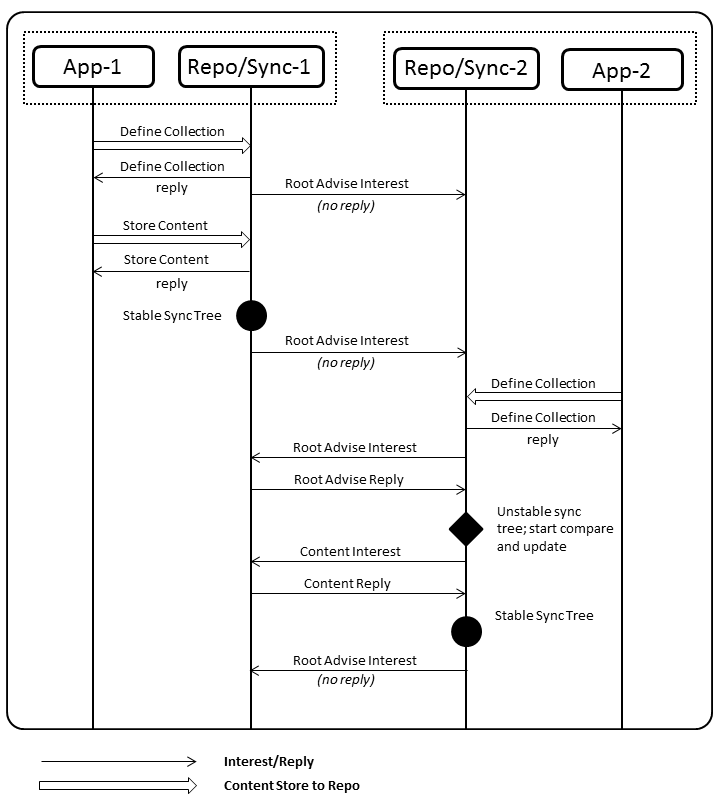
\includegraphics[scale=0.9]{./resources/figures/Sync.png}
\makebox[\textwidth][c]{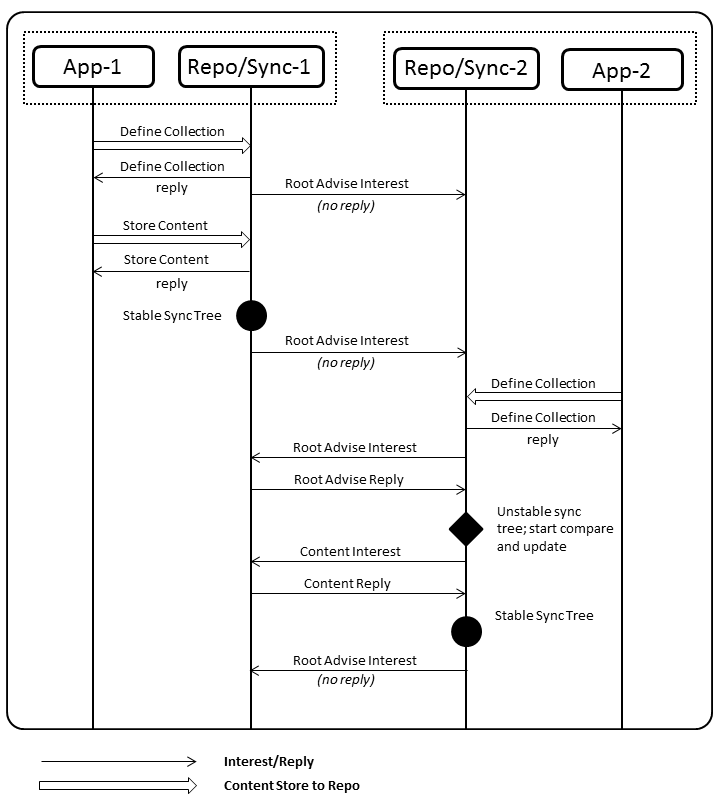
\includegraphics[width=1.1\textwidth]{./resources/figures/Sync.png}}%
\caption{نحوه‌ی انجام عملیات همگام‌سازی بین مجموعه‌های داده توسط عامل همگام‌ساز}
\label{fig:Sync1}
\end{figure}

عملیات همگام‌سازی در پروتکل Sync با استفاده از در‌هم‌سازی\زیرنوشت{Hash} انجام می‌گیرد. عامل همگام‌ساز برای هر درخت همگام‌سازی یک مقدار در‌هم‌ساز محاسبه می‌کند. این محاسبه به شکل بازگشتی انجام می‌گیرد. مقدار درهم‌ساز برای یک گره از درخت جمع جبری مقدار در‌هم‌ساز برای تک تک نام‌های آن گره و مقدار در‌هم‌ساز فرزندان آن است. در نتیجه مقدار در‌هم‌ساز برای کل درخت، در حقیقت جمع جبری تمام نا‌م‌های درون آن است. 

عامل همگام‌ساز برای همگام‌سازی مجموعه با مجموعه‌های متناظرش در مخازن مجاور، به طور دوره‌ای بسته‌ای به نام درخواست مشورت ریشه\زیرنوشت{Root Advise Interest} به عامل‌های همگام‌ساز همسایه می‌فرستد. این بسته حاوی مقدار درهم‌ساز درخت متناظر مجموعه است. عامل همگام‌ساز همسایه مقدار در‌هم‌ساز را با مقدار در‌هم‌سازی که خودش برای درخت مجموعه به دست آورده است مقایسه می‌کند. در صورتی که این دو مقدار مطابقت داشته باشند، پاسخی فرستاده نمی‌شود. در غیر این صورت، عامل همگام‌ساز همسایه در پاسخ مقدار در‌هم‌ساز ریشه‌ی خود را به همراه گره ریشه ارسال می‌کند. عام همگام‌ساز محلی با استفاده از درخواست واکشی گره\زیرنوشت{Node Fetch Interest} یکی پس از دیگری همه‌ی گره‌هایی که مقدار در‌هم‌سازشان با مقدار محاسبه‌شده توسط خودش مطابقت ندارد واکشی می‌کند تا به برگ‌هایی برسد که عامل این تغییر بوده اند، بدین معنی که در مجموعه‌ی همسایه وجود دارند ولی در مجموعه‌ی محلی خیر. سپس برای هر یک از این برگ‌ها یک بسته‌ی درخواست به همسایه‌ی خود می‌فرستد تا مجموعه‌ی محلی به‌روز شده و با مجموعه‌ی همسایه همگام شود.
 	
در شکل ~\ref{fig:Sync1} یک نمونه از همگام‌سازی را مشاهده می‌کنید. در این مثال دو برنامه‌ی App-1 و App-2 هر کدام از مخازن و عامل همگام‌ساز بهره می‌برند. ابتدا App-1 یک مجموعه‌ی جدید ایجاد می‌کند و تعدادی شی به آن اضافه می‌کند. در این میان پیغام‌های مشورت ریشه‌ای که بین دو عامل همگام‌ساز ردوبدل می‌شود با پاسخی روبه‌رو نمی‌شود و آن نیز به این دلیل است که در مخزن App-2 چنین مجموعه‌ای وجود ندارد و بنابراین مجموعه‌ای که در مخزن App-1 وجود دارد با خودش همگام است و درخت همگام‌سازی نیز پایدار است. پس از مدتی App-2 یک مجموعه با همان نام به مخزن خود اضافه می‌کند. از آن‌جایی که این مجموعه در مخزن App-2 خالی است ولی در مخزن App-1 اشیایی در آن وجود دارد، پیغام مشورت ریشه‌ای که از عامل همگام‌ساز App-2 به عامل همگام‌ساز App-1 فرستاده می‌شود، با پاسخی شامل مقدار درهم‌ساز درخت در مخزن App-1 روبه‌رو می‌شود. پس از آن عملیات همگام‌سازی به صورت مرحله به مرحله انجام می‌شود تا عامل همگام‌ساز App-2 داده‌های ناهمگون را پیدا کند. سپس عامل همگام‌ساز App-2 درخواست‌هایی برای دریافت محتوایی که ندارد به عامل همگام‌ساز App-2 می‌فرستد و داده‌های موردنظر را دریافت می‌کند. پس از این مرحله دو مجموعه با هم همگام خواهند بود و پیغام‌های مشورت ریشه باز هم بی‌پاسخ خواهند ماند.

لازم به ذکر است که هر درخواست مشورت ریشه دوره‌ی حیاتی دارد که با اتمام آن، درخواست مشورت ریشه‌ی جدیدی فرستاده می‌شود. این مسئله بدین منظور است که در صورت گم‌شدن  بسته‌های درخواست، عملیات همگام‌سازی با مشکل روبه‌رو نشود. اما در صورتی که فرکانس ارسال این درخواست‌ها زیاد باشد، سربار زیادی برای شبکه خواهد داشت. حالت ایده‌آل این خواهد بود که فرکانس ارسال این درخواست‌ها به صورت پویا و با توجه به وضعیت ترافیک شبکه تنظیم شود که نیاز به بررسی بیشتری دارد.

\زیرقسمت{Sync در پروتکل پیشنهادی}

در این قسمت نحوه‌ی استفاده از مخازن CCNx و پروتکل Sync برای توزیع بسته‌های مسیریابی را توضیح خواهیم داد. در پروتکل پیشنهادی دو نوع بسته باید توزیع شوند، بسته‌های مربوط به مسیرهای بین مسیریاب‌ها (DA)، و بسته‌های مربوط به توزیع پیشوندها (PA). از آنجایی که پیشوندها باید در سرتاسر شبکه توزیع شوند، در مخزن CCNx همه‌ی مسیریاب‌ها یک مجموعه با پیشوند \کج{<network>/RM/PA/} تعریف می‌کنیم تا تمام بسته‌های اعلام‌کننده‌ی پیشوند در این مجموعه ذخیره شوند. در نتیجه‌ی این کار هرگاه یک مسیریاب بخواهد یک پیشوند را اعلام کند، بسته‌ی PA مربوطه را با ساختار مشخص خود می‌سازد و به این مجموعه اضافه می‌کند. در نتیجه‌ی این کار مجموعه‌های دیگر از حالت همگام با این مجموعه خارج خواهند شد و پروتکل Sync برای پیدا کردن ناهمگونی‌ها بین عوامل همگام‌ساز مجاور اجرا می‌شود. با همگام شدن مجموعه‌ها، بسته‌ی جدید در مخزن تمام مسیریاب‌ها وجود خواهد داشت و در نتیجه بسته در شبکه پخش خواهد شد.

\begin{figure}[h!]
\centering
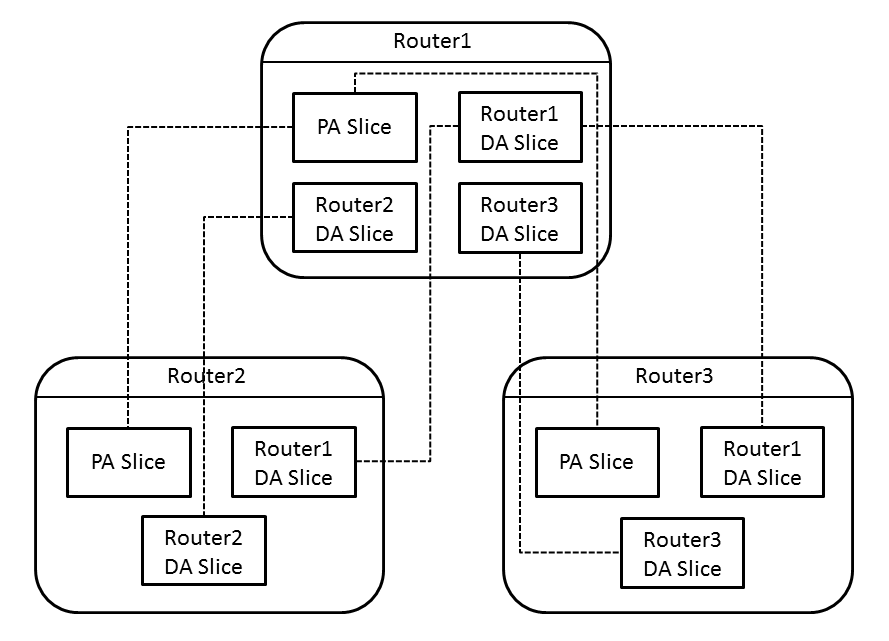
\includegraphics[scale=0.7]{./resources/figures/connection.png}
%\makebox[\textwidth][c]{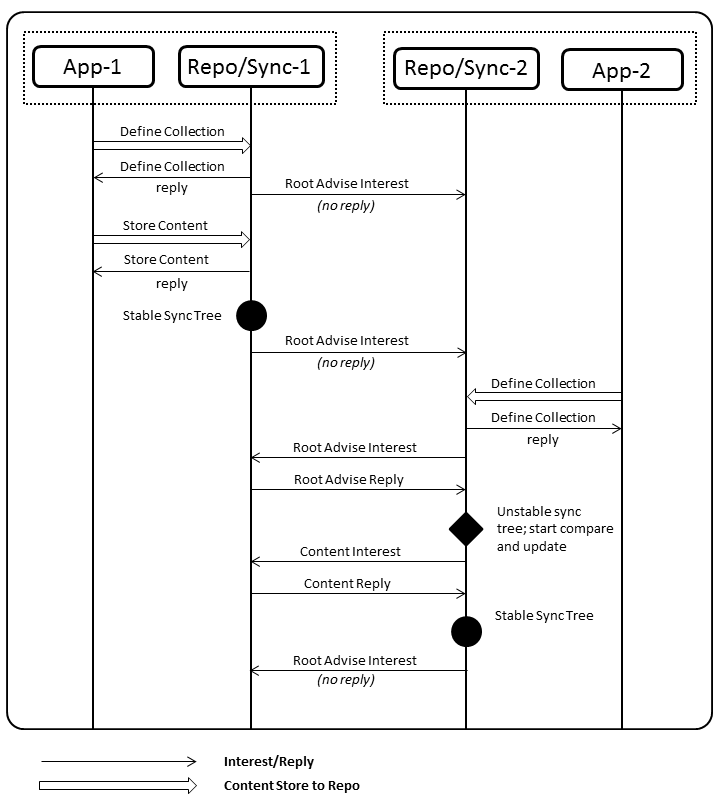
\includegraphics[width=1.1\textwidth]{./resources/figures/Sync.png}}%
\caption{مجموعه‌های داده‌ی تعریف شده برای ایجاد ارتباط بین مسیریاب‌های مجاور و تبادل بسته‌های مربوط به مسیریابی}
\label{fig:connection}
\end{figure}

مشابه این عملیات باید برای بسته‌های اعلام‌کننده‌ی فاصله (DA) نیز انجام شود. تفاوتی که این بسته‌ها با PAها دارند این است که نباید در سرتاسر شبکه توزیع شوند، بلکه هر مسیریاب بسته‌های DA را تنها به همسایه‌های خود ارسال می‌کند. همسایه‌ها پس از به‌روزرسانی FIB، در صورت نیاز خود بسته‌های DA جدیدی شامل هزینه‌های جدید به همسایه‌های خود می‌فرستند. به همین دلیل، هر مسیریاب باید یک مجموعه برای ارسال بسته‌های DA خود داشته باشد و آن را با همسایه‌های خود به اشتراک بگذارد. این مجموعه برای مسیریاب \کج{<router>} با نام \کج{/<network>/RM/<router>/DA}  مشخص می‌شود. با توجه به این توضیحات، هر مسیریاب به ازای هر یک از همسایه‌های خود یک مجموعه در مخزن خود خواهد داشت که نام آن همسایه در نام مخزن وجود دارد. 

در شکل ~\ref{fig:connection} مثالی از مجموعه‌های داده‌ی تعریف شده در مسیریاب‌ها برای تبادل بسته‌های DA و PA  نشان داده شده است. در این مثال Router1 با Router2 و Router3 همسایه است. مجموعه‌ی داده‌ی مربوط به PA ها با نام PA Slice بین هر سه مسیریاب مشترک است. علاوه بر آن هر مسیریاب مجموعه‌ی مخصوصی برای توزیع بسته‌های DA خود دارد که آن را به همسایگان خود به اشتراک می‌گذارد.

با وجود این که پروتکل Sync روش مناسبی برای همگام‌سازی دو مجموعه‌ی داده فراهم می‌کند، با مشکلاتی نیز روبه‌رو است. از جمله مشکلات این پروتکل که در مسیریابی به چشم می‌آید عدم پشتیبانی صحیح از حذف داده‌هاست. در مثال شکل ~\ref{fig:Sync1} فرض کنید پس از همگام‌شدن مجموعه‌های داده در مخازن App-1 و App-2، App-1 یکی از اشیا را پاک کند. در آن صورت اگر عامل همگام‌ساز در App-1 درخواست مشورت ریشه را برای عامل همگام‌ساز App-2 ارسال کند، متوجه می‌شود که داده‌ی پاک شده را در اختیار ندارد و حتی ممکن است دوباره آن را به مجموعه‌ی خود اضافه کند. هم‌چنین این امکان وجود دارد که عامل همگام‌ساز در App-2 درخواست مشورت ریشه را برای عامل همگام‌ساز App-1 ارسال کند و چون داده‌ای کم ندارد، تغییری در مجموعه‌ی داده‌ی خود ایجاد نکند. در حقیقت برخورد این پروتکل با حذف داده به طور قطعی و دقیق مشخص نیست. این مسئله در تبادل بسته‌های مسیریابی مشکل ایجاد می‌کند، زیرا با ایجاد نسخه‌های جدیدتر بسته‌های DA و PA، برای جلوگیری از انفجار داده‌های مجموعه‌ها، لازم است نسخه‌های قبلی از مجموعه‌های داده حذف شود. برای حل این مشکل برای دو نوع بسته‌ی PA و DA در عامل همگام‌ساز و پروتکل Sync تغییراتی ایجاد کرده‌ایم که در ادامه به آن‌ها خواهیم پرداخت.

از آن‌جایی که مجموعه‌ی مربوط به DA برای هر مسیریاب برای انتشار بسته‌های DA تولید شده توسط آن تعریف می‌شوند، تنها برنامه‌ای که نیاز دارد به مجموعه شی اضافه کند یا از آن حذف کند، خود مسیریاب است و نه همسایه‌های آن. بلکه برای همسایه‌های آن تنها کافی است که مجموعه‌ی خود را با آن همگام کنند، پیغام‌های درون مجموعه‌ی داده بخوانند، و FIB خود را بر اساس آن به‌روزرسانی کنند. به همین دلیل تنها مسیریابی می‌تواند در یک مجموعه‌ی داده‌ی مربوط به DA بنویسد که نام آن در نام مجموعه‌ی داده وجود دارد. در نتیجه، عامل‌های همگام‌ساز همسایه‌ها را به گونه‌ای تغییر می‌دهیم تا در اجرای پروتکل Sync هنگامی که متوجه می‌شوند که داده‌ای از مجموعه‌ی داده حذف شده است، آن را از مجموعه‌ی داده‌ی خود حذف کنند. هم‌چنین یک عامل همگام‌ساز یک مسیریاب در صورتی که در اجرای پروتکل Sync متوجه شد که مجموعه‌ی داده‌ی مخصوص خودش برای بسته‌های DA، از مجموعه‌های داده‌ی همسایگان داده‌ای کم دارد، آن را اضافه نمی‌کند، بلکه منتظر می‌ماند که آن‌ها داده را از مجموعه‌ی خود حذف کنند تا مقدار درهم‌ساز در درخواست‌های بعدی مشورت ریشه یکی شود. 

در مورد بسته‌های PA موضوع اندکی متفاوت است. از آن‌جایی که هر مسیریابی می‌توانند به تولید و انتشار بسته‌های PA بپردازد، نمی‌توان مسئله‌ی حذف را با محدود کردن حق شروع تغییر به یک مسیریاب، حل کرد. به همین دلیل هر گاه مسیریابی بخواهد یک بسته‌ی PA را از مجموعه‌ی داده‌ی مربوط به آن حذف کند، علاوه بر حذف آن، یک بسته با همان نام که یک \کج{/delete} به انتهای آن اضافه شده است و با همان محتوا به مجموعه اضافه خواهد کرد. حال در صورتی که در اجرای پروتکل Sync یکی از عامل‌های همگام‌ساز متوجه شود که مجموعه‌ی داده‌ی آن، داده‌ای کمتر از مجموعه‌ی داده‌ی همسایه دارد، ابتدا بررسی می‌کند که داده‌ای با همان نام و پسوند \کج{/delete} در مجموعه‌ی همسایه وجود دارد یا نه. البته توجه به این نکته ضروری است که داده‌های اضافه‌تر مجموعه‌ی همسایه در حین اجرای پروتکل اصلی Sync مشخص خواهند شد. در صورتی که چنین داده‌ای وجود داشته باشد، عامل همگام‌ساز داده‌ی موردنظر یا همان بسته‌ی PA حذف شده را از مجموعه‌ی داده‌ی خود حذف خواهد کرد. از طرفی اگر عامل همگام‌ساز مسیریابی که بسته را حذف کرده، در حین اجرای پروتکل متوجه شد که داده‌ای کمتر از مجموعه‌ی داده‌ی همسایه دارد، وجود داده‌ای با همان نام و پسوند \کج{/delete} را بررسی خواهد کرد و در صورت وجود این داده، داده‌ی حذف شده را از مجموعه‌ی همسایه واکشی نخواهد کرد.

\begin{figure}[h!]
\centering
%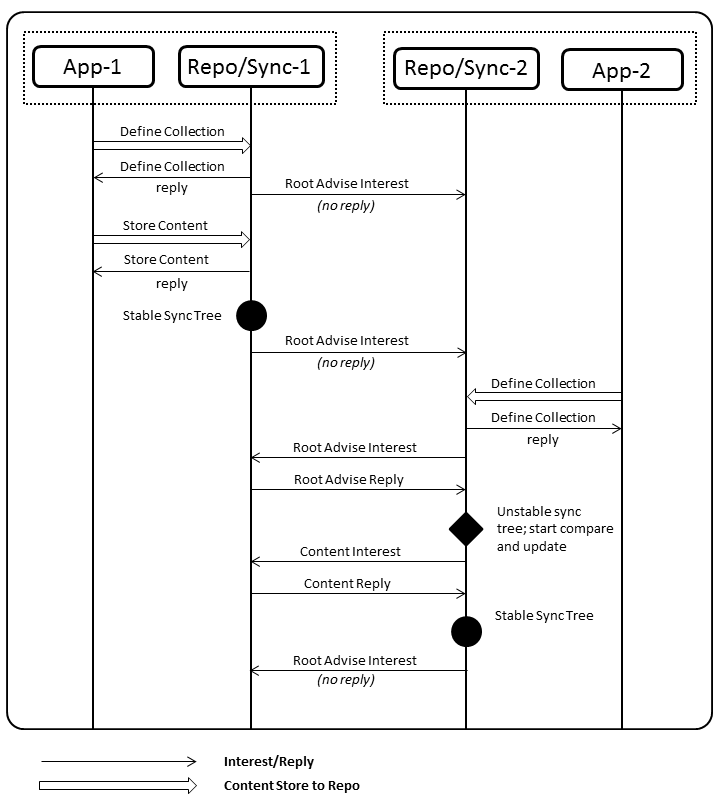
\includegraphics[scale=0.9]{./resources/figures/Sync.png}
\makebox[\textwidth][c]{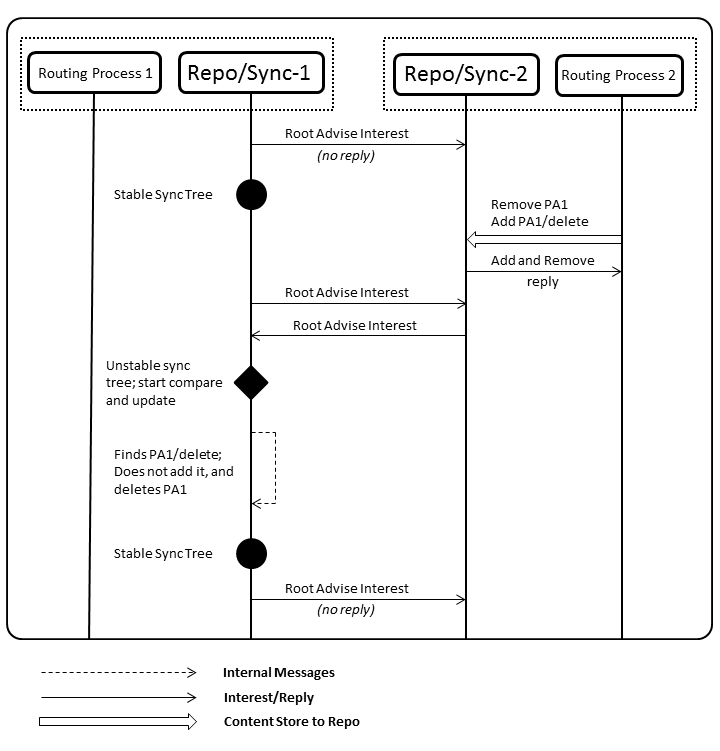
\includegraphics[width=1.1\textwidth]{./resources/figures/Sync2.png}}%
\caption{نحوه‌ی انجام عملیات حذف یک بسته‌ی اعلام‌کننده‌ی پیشوند از مجموعه‌ی داده}
\label{fig:Sync2}
\end{figure}


نکته‌ای که در مورد داده‌های با پسوند \کج{/delete} وجود دارد این است که این بسته‌ها در مجموعه‌ی داده باقی می‌مانند. برای جلوگیری از انفجار مجموعه‌های داده در بازه‌های مشخص هر مسیریاب داده‌های با پسوند \کج{/delete} موجود در مجموعه‌های داده‌ی خود را پاک خواهد کرد. بنابراین در صورتی که در یک اجرای پروتکل Sync، یک عامل همگام‌ساز متوجه شد که مجموعه‌ی داده‌ی آن در تنها در یک داده با پسوند \کج{/delete} با مجموعه‌ی داده‌ی همسایه متفاوت است، یعنی داده‌ی اصلی و بدون پسوند را ندارد ولی همان داده با پسوند \کج{/delete} در مجموعه‌ی همسایه وجود دارد، بسته‌ی با پسوند \کج{/delete} را واکشی نخواهد کرد. بدین‌ترتیب داده‌های با پسوند \کج{/delete} که در واقع همان بسته‌های اعلام‌کننده‌ی پیشوند حذف‌شده هستند، در مجموعه‌ی داده‌ها باقی نخواهند ماند. شکل ~\ref{fig:Sync2} نمونه‌ای از حذف یک بسته‌ی PA را از مجموعه‌ی داده‌ی مربوط به آن نشان می‌دهد. 


\قسمت{کشف شکست و ترمیم}

برای اطمینان در درستی پیوند یا پردازه‌ی مسیریاب در گره همسایه، مشابه بسیاری از پروتکل‌های دیگر، هر مسیریاب در بازه‌های مشخصی از زمان بسته‌های درخواست سلام\زیرنوشت{Hello Interest} به هر یک از همسایه‌های خود می‌فرستد. همسایه نیز در صورت دریافت یک درخواست سلام، آن را با بسته‌ی داده‌ی سلام\زیرنوشت{Hello Data} پاسخ خواهد داد. در صورتی که یک درخواست سلام، با پاسخی مواجه نشود، مسیریاب چند بار دیگر در بازه‌های کوتاه‌تری با فرستادن بسته‌های درخواست برای برقراری ارتباط تلاش می‌کند و در صورتی که موفق نشود، پیوند را غیرفعال فرض می‌کند، FIB را به‌روزرسانی می‌کند و در صورت تغییر بهترین مسیرش تا سایر مسیریاب‌ها پیغام‌های DA مربوطه را به همسایگانش می‌فرستد. 

برای اطلاع از ترمیم یک پیوند غیرفعال، مسیریاب در بازه‌های طولانی‌تری با فرستادن بسته‌های درخواست سلام فعال شدن پیوند را بررسی می‌کند. این بازه‌ها طولانی انتخاب می‌شوند تا سربار زیادی برای شبکه نداشته باشند. در صورتی که یک پیوند فعال شود، مسیریاب FIB خود را به روز‌رسانی می‌کند و در صورتی که استفاده از این پیوند فعال‌شده مسیرهای بهتری را برایش امکان‌پذیر کرده باشد، پیغام‌های DA مربوطه را به همسایگانش ارسال می‌کند.

\قسمت{مسئله‌ی شمارش بی‌انتها}

یکی از مشکلاتی که در مسیریابی‌های مبتنی بر بردار فاصله وجود دارد مسئله‌ی شمارش بی‌انتهاست که در بخش ؟؟؟‌ به آن اشاره شد. برای مقابله با این مسئله در پروتکل پیشنهادی خود، روشی مشابه پروتکل RIP\زیرنوشت{Routing Information Protocol} در پیش گرفته‌ایم. در این روش که سم معکوس\زیرنوشت{Poison Reverse} نامیده می‌شود، اگر مسیریاب «الف» بهترین مسیر خود به مسیریاب «ب» را از طریق مسیریاب «پ» در همسایگی خود داشته باشد، برای جلوگیری از شمارش بی‌انتها، فاصله‌ی خود از مسیریاب «ب» را به مسیریاب «پ» بی‌نهایت اعلام خواهد کرد. به عبارت دیگر، یک مسیریاب، مسیری که از همسایه‌ی خود فراگرفته است، به خود او تبلیغ نخواهد کرد. 

لازم به ذکر است که سم معکوس تنها مشکل را بین دو مسیریاب حل خواهد کرد و امکان بروز مشکل مشابه با بیش از دو مسیریاب نیز وجود دارد. برای رفع این مشکل به طور کلی پروتکل‌های مبتنی بر بردار فاصله‌ی دیگری نیز برای مسیریابی در شبکه‌های مبتنی بر IP به وجود آمده‌اند که پیچیدگی زیاد آن‌ها، استفاده از این پروتکل‌ها را با مشکل مواجه می‌کند. به همین دلیل، در پروتکل پیشنهادی خود تنها به استفاده از سم معکوس بسنده می‌کنیم. هم‌چنین برای کم کردن اثر شمارش بی‌انتها بر زمان همگرایی، مشابه پروتکل RIP، در زمان پیکربندی بیشینه‌ی فاصله با توجه به ویژگی‌های شبکه برای الگوریتم مسیریابی تعیین می‌شود تا فاصله‌های بیشتر از آن را بی‌نهایت در نظر بگیرد و در نتیجه شمارش بی‌انتها زودتر به نهایت برسد و پایان یابد. 

نکته‌ی قابل‌توجه دیگر در زمینه این است که مسئله‌ی شمارش بی‌انتها در شبکه‌های NDN به اندازه‌ی شبکه‌های مبتنی بر IP مشکل‌ساز نخواهد بود. دلیل این امر، ویژگی‌های خاص دامنه‌ی ارسال در شبکه‌های NDN است که در ~\ref{routing-forwarding}  به آن اشاره شد. دامنه‌ی ارسال در NDN کارایی مسیرهای مختلف رسیدن به یک داده را به صورت پویا زیر نظر می‌گیرد و با توجه به آن، واسط‌ها را رتبه‌بندی می‌کند. در نتیجه در مدتی که شبکه در حال همگرایی است و شمارش بی‌انتها در حال رخ‌دادن است، با وجود این که ممکن است هزینه‌ی به دست آمده برای مسیر موردنظر هنوز پایدار نشده باشد و مقدار مناسبی نداشته باشد، دامنه‌ی ارسال با مشاهده‌ی کارایی کم آن بسته‌ها را از آن مسیر ارسال نخواهد کرد. 
